\documentclass[style=upen, size=14pt]{powerdot}
\usepackage{natbib}
\usepackage{bibentry}
\usepackage{mathtools}
\definecolor{arany}{RGB}{255,242,0}
\hypersetup{backref=page}
\hypersetup{
    colorlinks=true,
    linkcolor=cyan,
    citecolor=cyan,
    filecolor=magenta,      
    urlcolor=cyan}
% \pdsetup{trans=Split}
\usepackage{graphicx}
\usepackage{amsmath}
\DeclareMathOperator*{\argmax}{argmax}
\DeclareMathOperator*{\argmin}{argmin}
\DeclareMathOperator*{\softmax}{softmax}
\DeclareMathOperator{\sign}{sign}
\usepackage{graphicx,wrapfig,lipsum}
\usepackage{amssymb}
\usepackage{stmaryrd}
\usepackage[latin2]{inputenc}
%\usepackage[magyar]{babel}
%\usepackage{euler}
\usepackage{tikz}
\usetikzlibrary{matrix}
\usepackage{tikz-qtree}
\usepackage{tikz-dependency}
\usepackage{linguex}
\usepackage{amsthm}
\usepackage{amsmath}
%\tikzset{every tree node/.style={align=center,anchor=north}}
%\usepackage{tabularx}
%\usepackage{threeparttable}
%\usepackage{color}
%\selectlanguage{english}
%\frenchspacing
\usepackage{algpseudocode}
\usepackage{algorithm}
\newcommand\varlist{,\makebox[1em][c]{.\hfil.\hfil.},}
\newcommand{\nd}{\noindent}
\newcommand{\Val}{\mathop{\mathit{Val}}}
\newcommand{\gold}{\color{arany}}
%\usepackage{tikz}
%\usepackage{tikz-qtree}
%\newcommand{\qed}{\hfill\mbox{\raggedright \rule{.1in}{.1in}}}
\def\es{\mathbin\land}
\theoremstyle{definition}
\newtheorem*{definition}{Definition}
\newtheorem{axioma}{Axiom}
\newtheorem{tetel}{Theorem}
\newtheorem{prop}{Proposition}
\newtheorem{lemma}{Lemma}
\begin{document}

\title{Natural Language Processing\\~~\\Lecture 7\\Lexical semantics}
% \author{}

\date{2021}
\maketitle

\begin{slide}[toc=]{FLAIR cont.}
  \begin{center}
    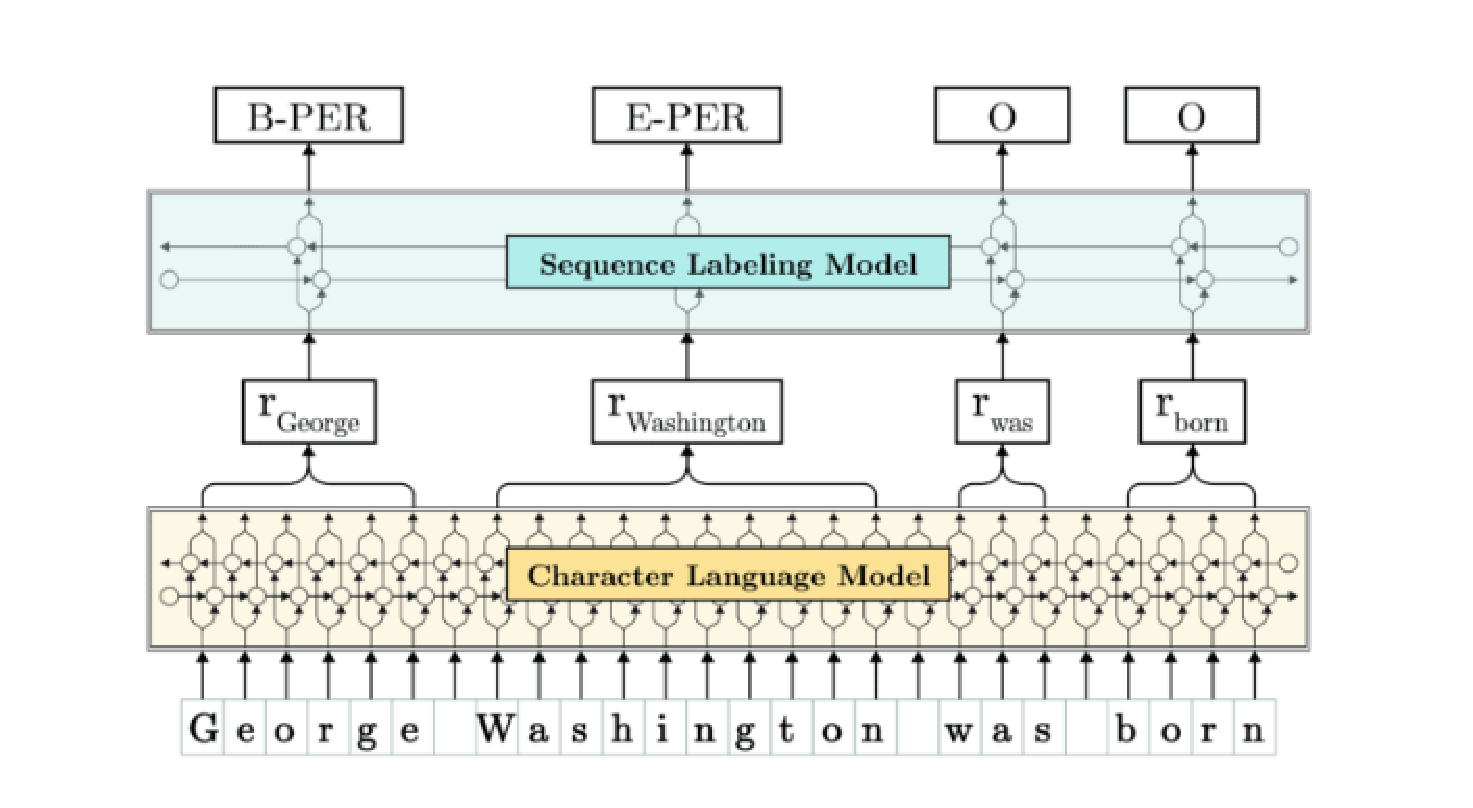
\includegraphics[width=1\textwidth]{figures/flair.eps}
    \footnotesize{(Figure from \cite{akbik2018contextual}).}
  \end{center}
\end{slide}

\section[toc=Transformers]{Interlude: Transformers}

\begin{slide}[toc=Introduction]{Contextual embeddings and transformers}
  The first contextual embeddings were produced by RNNs, but later developments
  were made possible by the discovery of \emph{\gold transformers}
  \citep{vaswani2017attention}, a new type of architecture using attention
  mechanisms as full-fledged layers, not as auxiliary RNN components.\bigskip

  Before discussing the recent transformer-based embedding models, we discuss
  shortly this new architecture and its building blocks:
  \begin{itemize}
  \item attention as soft dictionary lookup,
  \item self-attention layers, and
  \item transformer modules.
  \end{itemize}
\end{slide}

\begin{slide}[toc=KV-attention]{Attention as soft dictionary lookup}
  Recall that attention mechanisms provide \emph{query-based aggregation} of an
  $\langle \mathbf{x}_1,\dots, \mathbf{x}_n\rangle $ vector sequence: given an
  $\mathbf{x^*}$ \emph{query vector}, they calculate a sequence of relevance
  scores
  $$
  \mathbf{s} = \langle s(\mathbf{x}_1, \mathbf{x}^*),\dots, s(\mathbf{x}_n,
  \mathbf{x}^*) \rangle
  $$
  and returned the weighted sum 
  $$
  \softmax (\mathbf{s})\cdot \langle \mathbf{x}_1,\dots, \mathbf{x}_n\rangle 
  $$
  as a summary or aggregation of the $\mathbf{x}_i$-s according to their
  relevance score.
\end{slide}

\begin{slide}[toc=]{Attention as soft dictionary lookup cont.}
  The $s(\cdot, \cdot)$ scoring function varies, we saw that one option is to
  use the scaled dot-product:
  $$
  s(\mathbf{x}_i, \mathbf{x}^*) = \frac{\mathbf{x}_i\cdot
    \mathbf{x}^*}{\sqrt{d}}.
  $$
  where $d$ is the dimensionality of $\mathbf{x_i}$ and $\mathbf{x^*}$.\bigskip

  Building on this schema, the transformer attention mechanism makes a crucial
  change: treats $\langle \mathbf{x}_1,\dots, \mathbf{x}_n\rangle$ as a
  \emph{\gold dictionary}, for which there are $\mathcal K(\cdot)$ and $\mathcal V(\cdot)$
  mappings that map each $\mathbf{x}_i$ to a corresponding
  $\mathcal K(\mathbf{x}_i)$ key and $\mathcal V(\mathbf{x}_i)$ value.
\end{slide}


\begin{slide}[toc=]{Attention as soft dictionary lookup cont.}
  Assuming also a $\mathcal Q(\cdot)$ \emph{\gold query} mapping which maps
  $\mathbf{x}^*$ to the range of $\mathcal K$(.) (the ``key-space''), scoring
  can be reformulated as calculating dot-product based similarity scores between
  the query and keys
  $$
  s(\mathbf{x}_i, \mathbf{x}^*) = \frac{\mathcal K (\mathbf{x}_i)\cdot
    \mathcal Q (\mathbf{x}^*)}{\sqrt{d}},
  $$
  ($d$ is now the dimensionality of the ``key-space'') and the retrieved value
  will be the weighted sum
  $$
  \softmax(\langle
  s(\mathbf{x}_1,\mathbf{x}^*),\dots,s(\mathbf{x}_n,\mathbf{x}^*) \rangle)\cdot
  \mathcal V(\langle \mathbf{x_1},\dots,\mathbf{x}_n)\rangle.
  $$
\end{slide}

\begin{slide}[toc=Attention layer]{Attention as a layer cont.}
  The outlined attention mechanism can be used as a standalone layer for
  transforming an input vector sequence
  $\mathbf{I} = \langle \mathbf{i}_1,\dots, \mathbf{i}_n \rangle$:\bigskip

  Given another $\mathbf{X} = \langle \mathbf{x}_1,\dots, \mathbf{x}_m \rangle$
  sequence and $\mathcal K(\cdot),\mathcal V(\cdot),\mathcal Q(\cdot)$ mappings,
  for each $\mathbf{i_k}$ input, we can calculate the corresponding
  $\mathcal Q(\mathbf{i}_k)$ query, and use this with $\mathcal K$ and
  $\mathcal V$ to \emph{attend to} $\mathbf{X}$ and compute a corresponding
  attention response $\mathbf{o}_k$.\bigskip

  The result is an $\mathbf{O}=\langle \mathbf{o}_1,\dots,\mathbf{o}_n \rangle$
  sequence of outputs, which collectively is the layer's output for the input
  $\mathbf{I}$.
\end{slide}

\begin{slide}[toc=]{Attention as a layer cont.}
  Depending on where the layer attends to (where $\mathbf{X}$ comes from) we can
  distinguish self- and outward attention layers.
  \begin{itemize}
  \item In \emph{\gold self-attention} layers, the queries generated from the
    input are used to query the input iself: $\mathbf{X}=\mathbf{I}$.
  \item In an \emph{\gold outward} attention layer, an external vector sequence
    is queried, e.g., in encoder-decoder transformer architectures a sequence
    created by an encoder.
  \end{itemize}
  As for the mappings $\mathcal K(\cdot),\mathcal V(\cdot),\mathcal Q(\cdot)$,
  all three are commonly implemented as \emph{\gold linear projections}, with
  learned weight matrices $W_K, W_V, W_Q$.
\end{slide}

\begin{slide}[toc=Multiple heads]{Multi-headed attention}
  To able to attend to multiple aspects of the input, the attention layers in
  transformers contain several parallel attention ``heads'' with different
  $W_K, W_V, W_Q$ triplets:
  
  \hspace{0.6cm}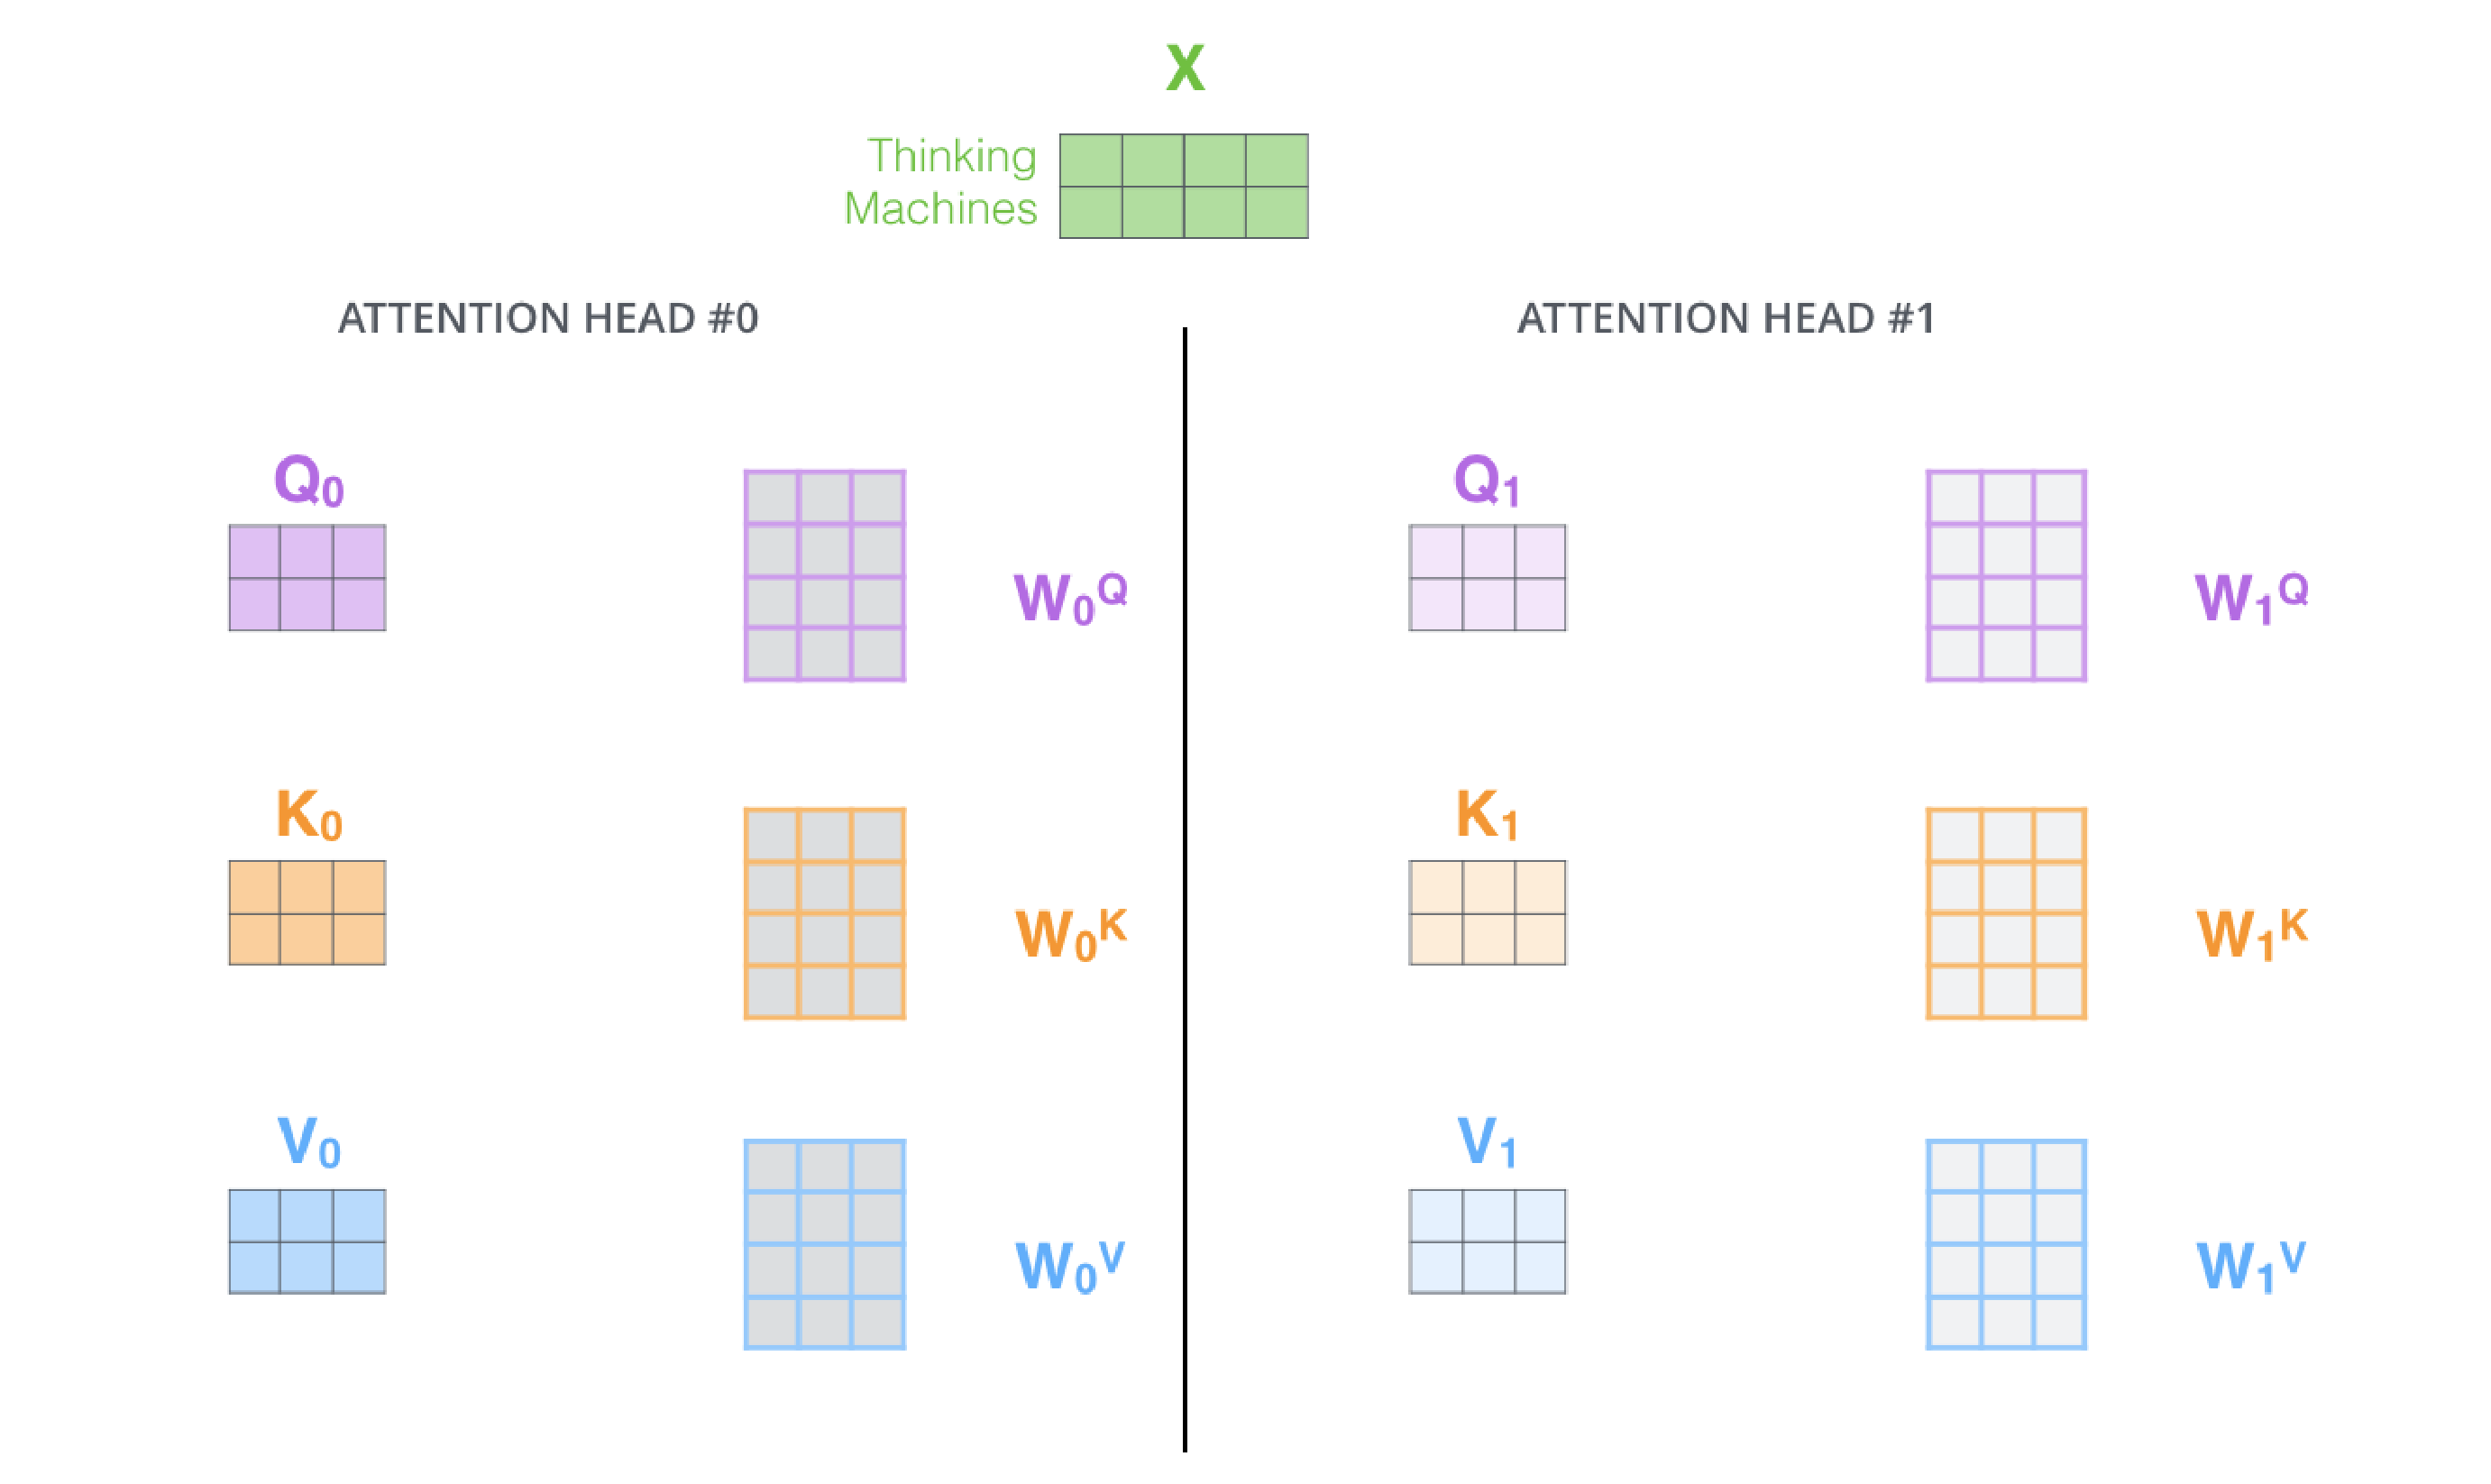
\includegraphics[width=0.9\textwidth]{figures/transformer_attention_heads_qkv.eps}
    
  \hspace{3cm}\footnotesize{(Figure from \cite{alammar2018illustrated}.)}
\end{slide}

\begin{slide}[toc=]{Multi-headed attention cont.}
  The head outputs are combined into a layer output:

  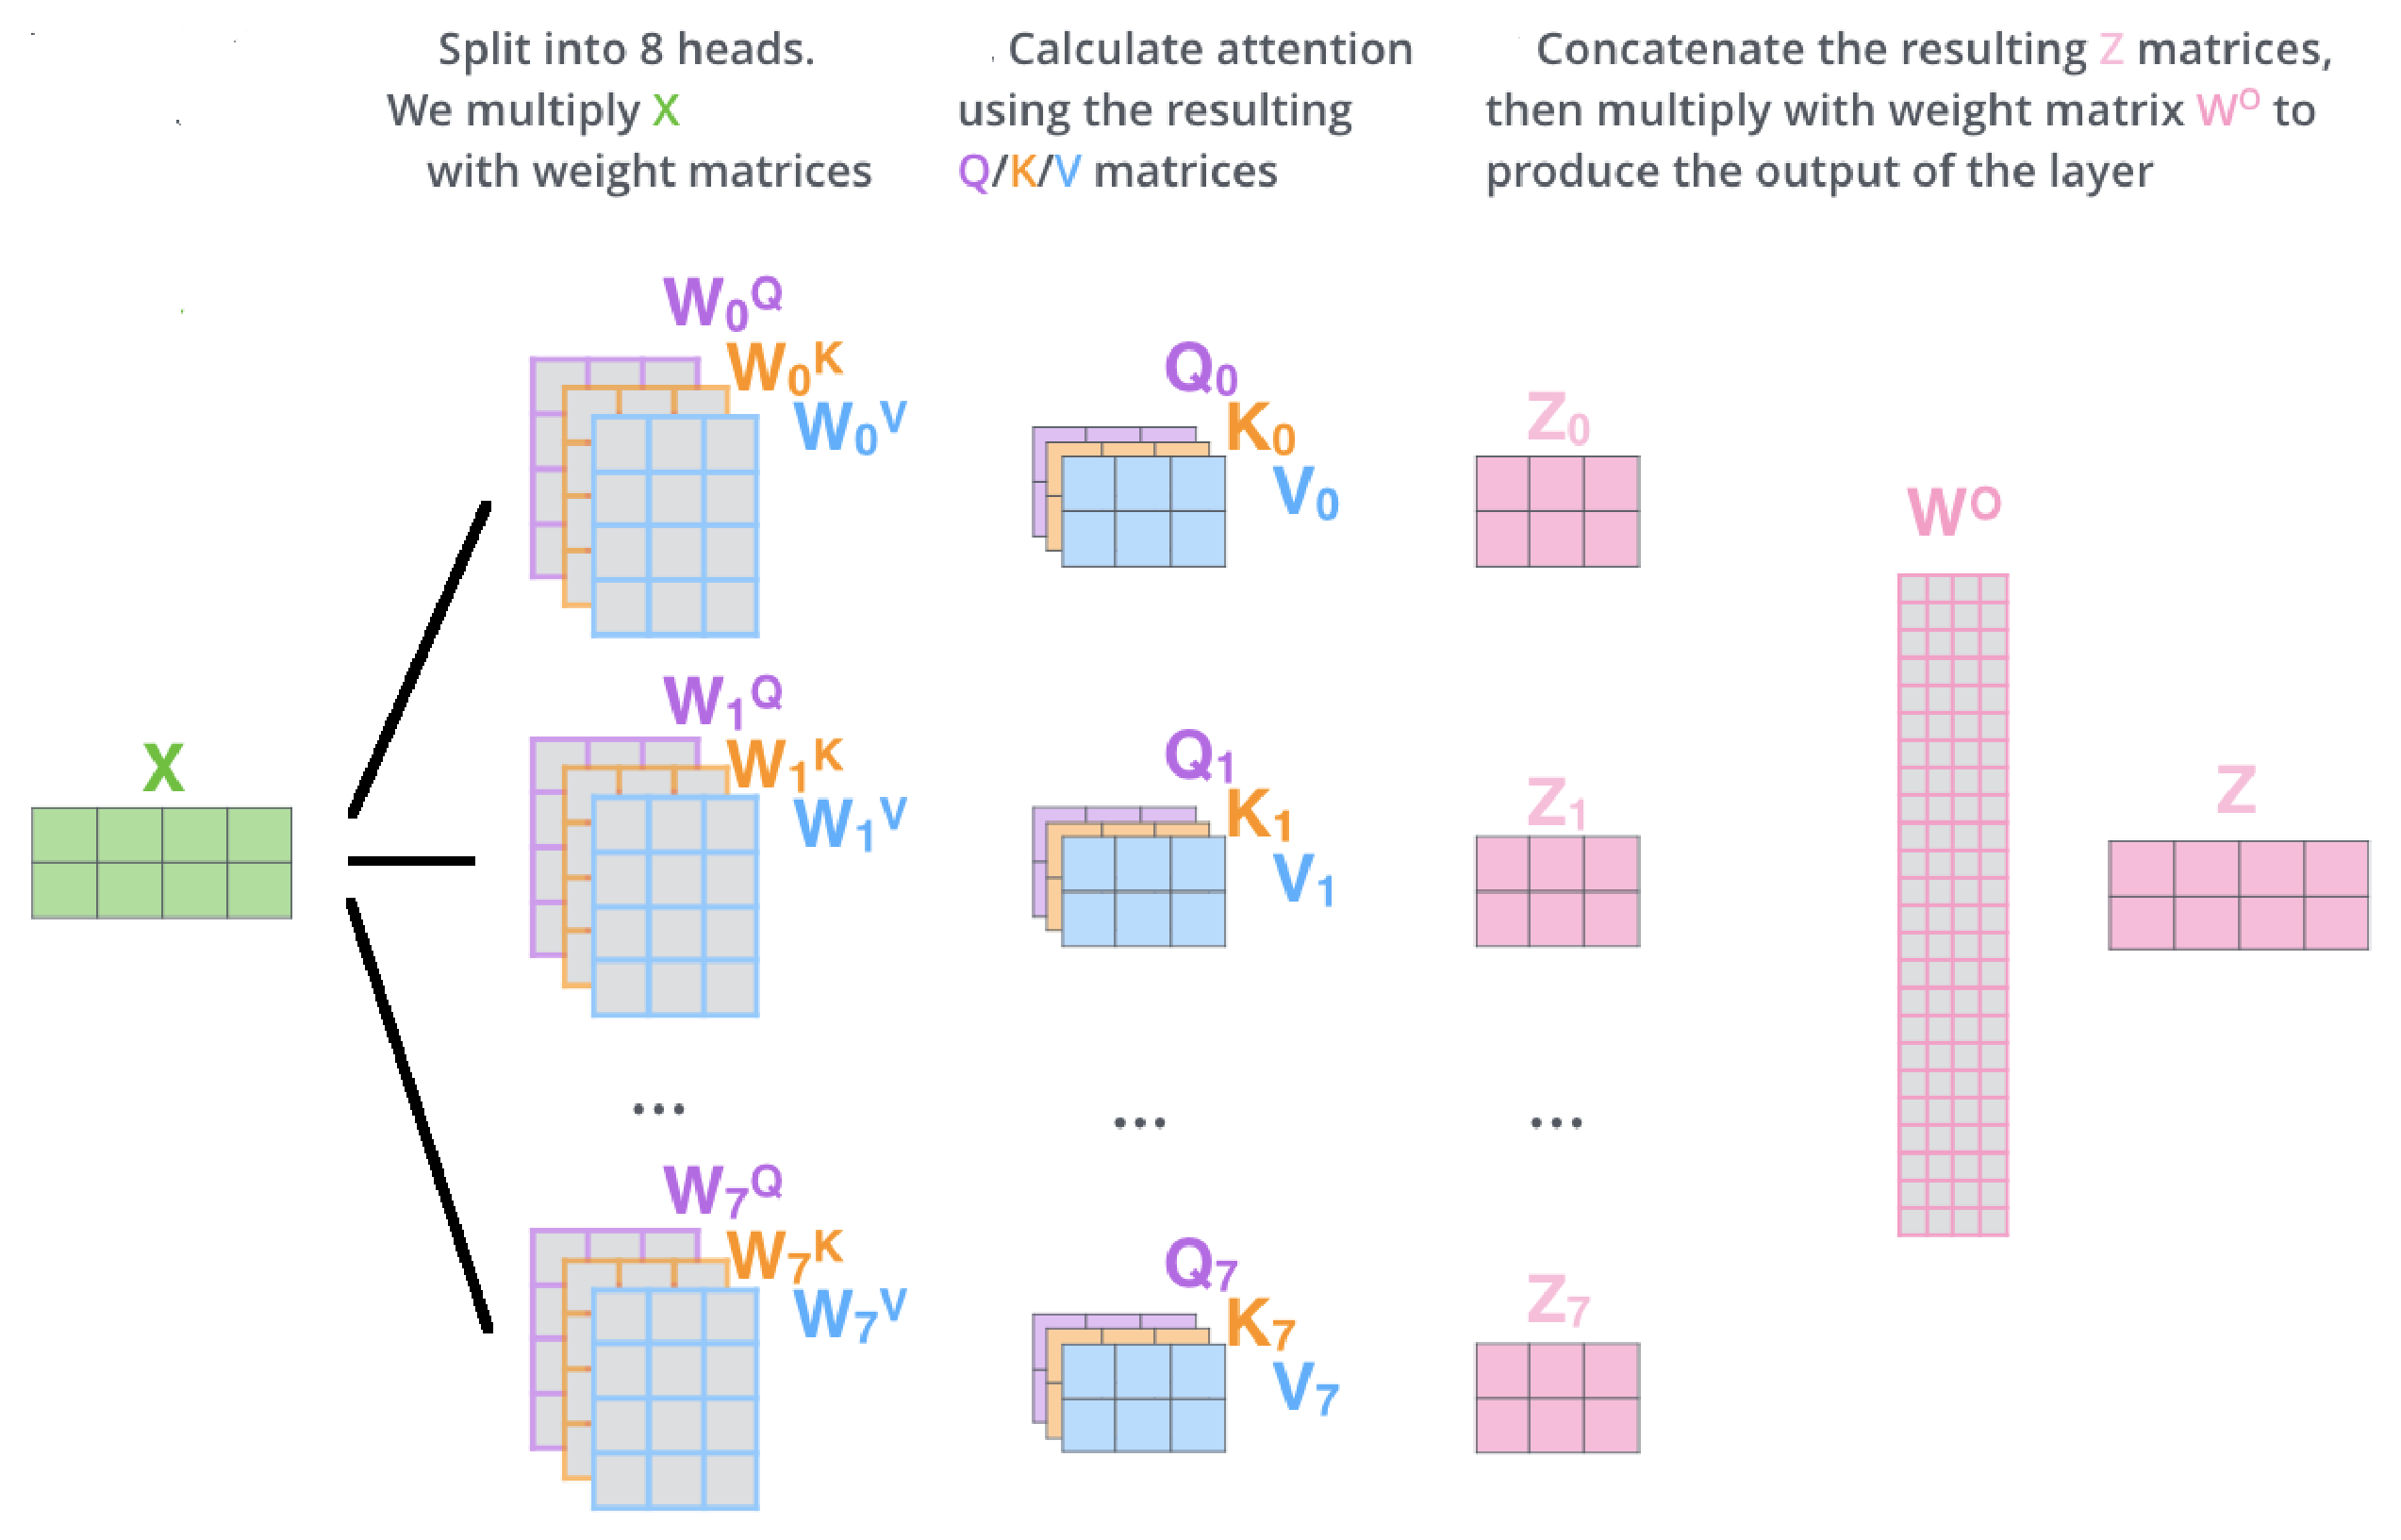
\includegraphics[width=1\textwidth]{figures/mhead2.eps}    

  \hspace{3cm}\footnotesize{(Figure adapted from
    \cite{alammar2018illustrated}.)}
\end{slide}

\begin{slide}[toc=Modules]{Transformer modules}
  The building blocks of transformers are \emph{\gold transformer modules}
  consisting of attention and simple piecewise feedforward layers. The simplest
  variant contains only a single self-attention layer:
  
  \begin{centering}
    
    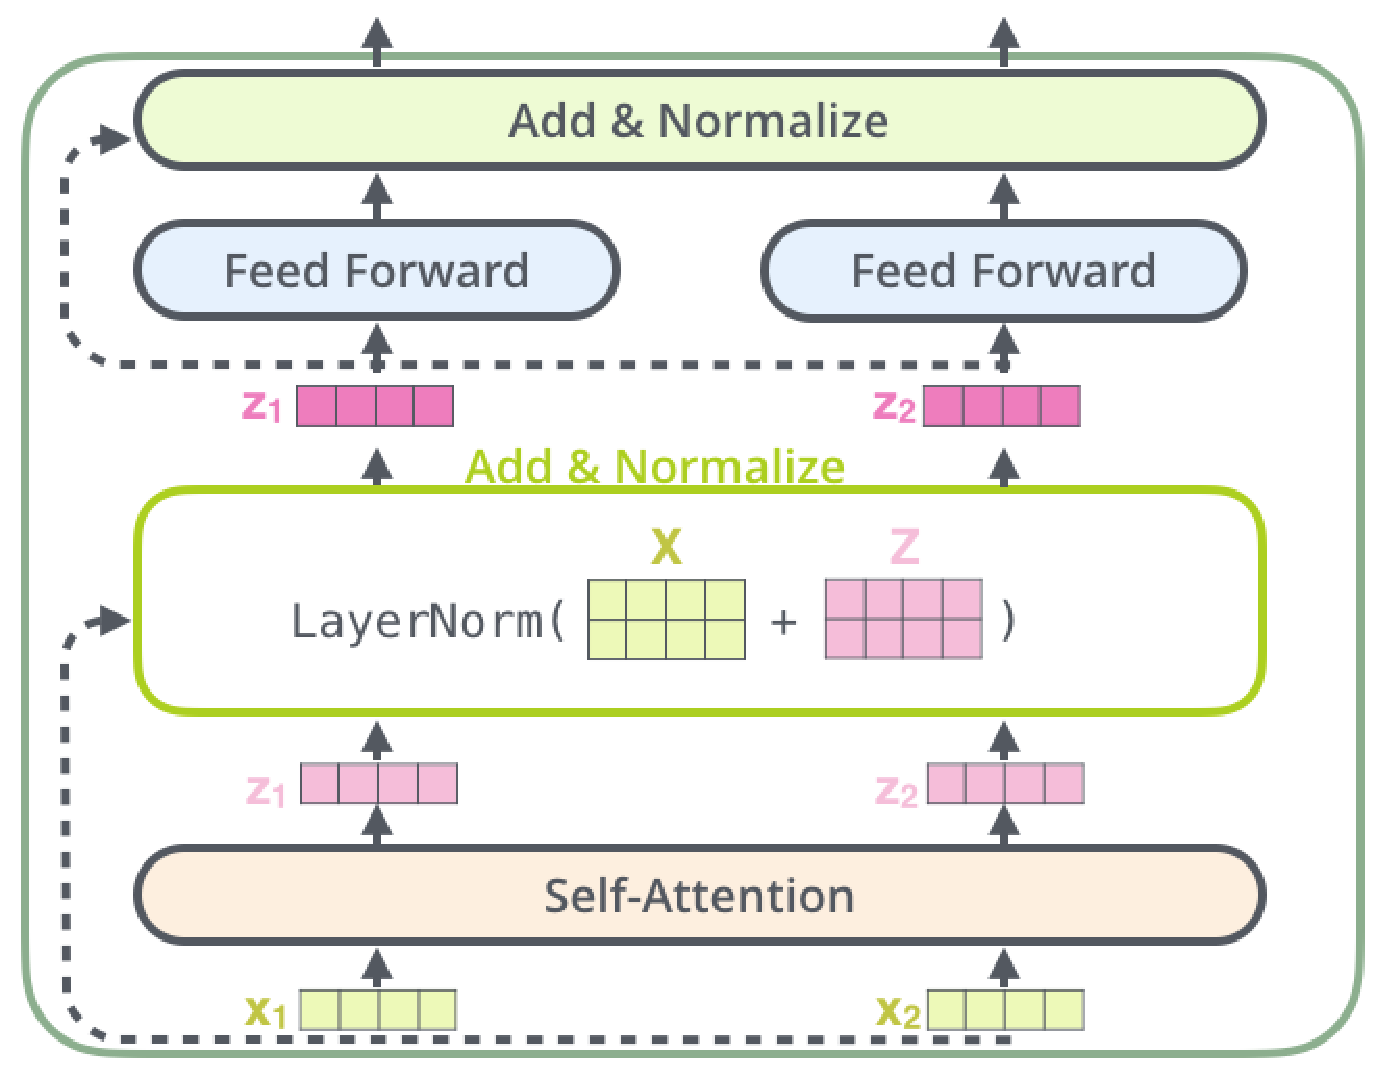
\includegraphics[width=0.6\textwidth]{figures/transformer_resideual_layer_norm_2.eps}

    \footnotesize{(Figure adapted from \cite{alammar2018illustrated}.)}
    
  \end{centering}
\end{slide}

\begin{slide}[toc=]{Transformer modules cont.}
  \begin{wrapfigure}{r}{3.5cm}
    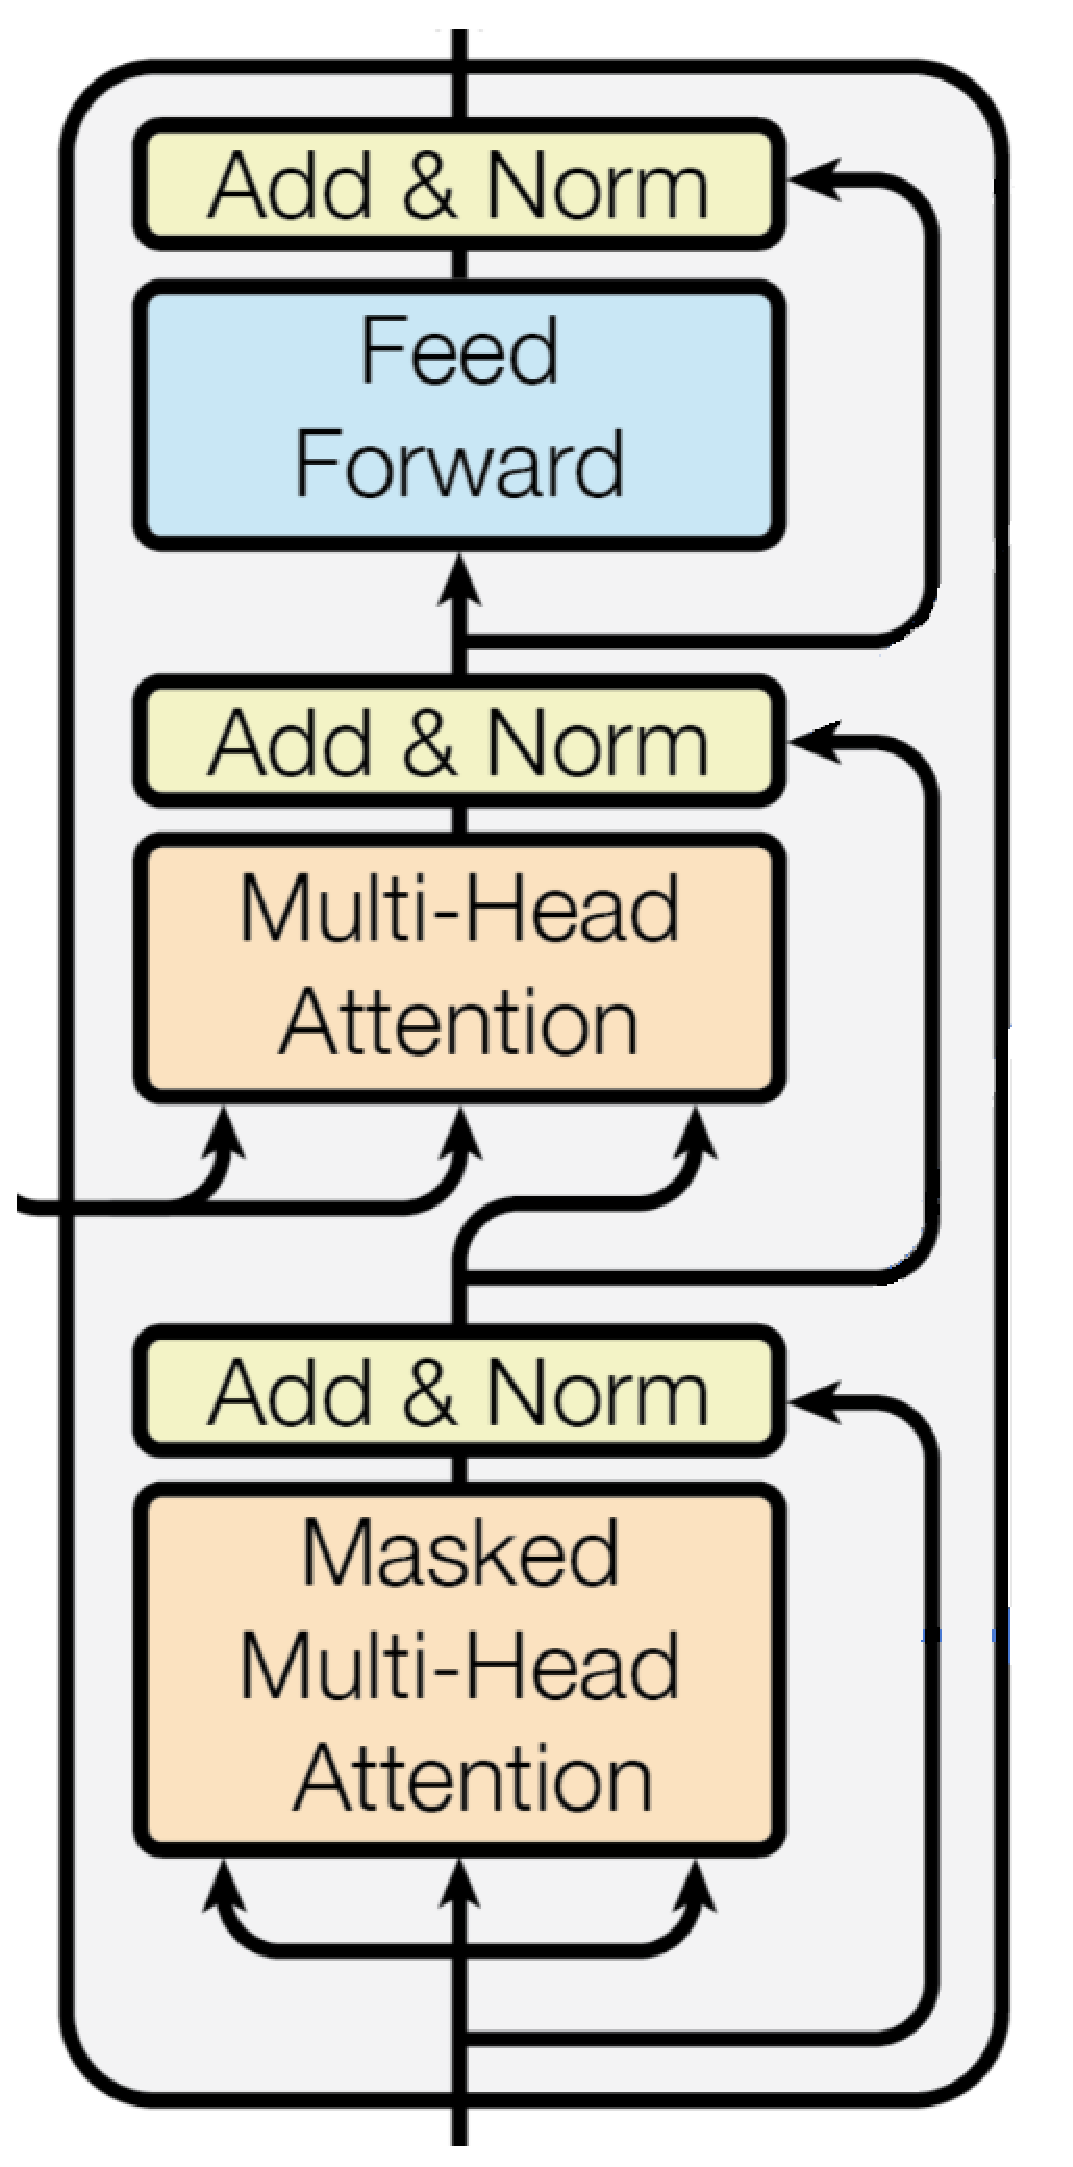
\includegraphics[width=3.5cm]{figures/transformer_block.eps}
  \end{wrapfigure}
  The \emph{decoder} part of transformers is built from more complex modules: in
  addition to a self-attention layer, they also contains an outward attention
  layer, which attends to the output of the model's encoder. The self-attention
  layer is \emph{masked}: attention queries from a decoder position cannot
  access information in later decoder positions to not use ``future
  information'' during training with teacher forcing.\medskip

  \footnotesize{(This and the next figure from \cite{vaswani2017attention}.)}
\end{slide}

\begin{slide}[toc=Seq2seq]{Seq2seq transformer}
    \begin{wrapfigure}{r}{4.8cm}
    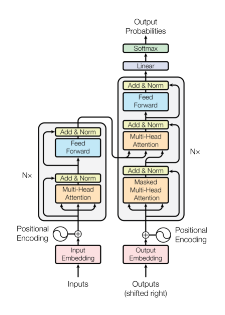
\includegraphics[width=4.8cm]{figures/transformer_full.eps}
  \end{wrapfigure}
  The original \emph{full transformer model} of \citep{vaswani2017attention} was
  a Seq2seq encoder-decoder model built exclusively of transformer blocks.
  During inference the decoder part predicts step-by-step, consuming already
  predicted output similary to RNNs, but during training it requires only a
  single forward pass with teacher forcing.
\end{slide}

\section{Transformer-based contextual embeddings}

\begin{slide}[toc=Introduction]{Transformer-based embeddings}
  The transformer architecture was first used for translation (2017), but
  starting from 2018, a series of transformer-based models producing contextual
  embeddings were developed. The most important research areas were
  \begin{itemize}
  \item finding self-supervised tasks conducive to learning high-quality
    representations;
  \item architectural improvements, importantly, finding more efficient attention variants;
  \item how to adapt/fine-tune the pretrained representation networks for
    downstream tasks.
  \end{itemize}
\end{slide}

\begin{slide}[toc=GPT]{GPT (Generative Pre-Training, OpenAI, 2018)}
  GPT is a BPE-based, decoder only transformer model trained with a
  traditional "predict the next token" language modeling objective. The
  contextual embeddings are simply the outputs of the top transformer module.\bigskip

  Similarly to ELMo, the main goal of GPT is to provide a useful pretrained
  "feature extractor" module, which can be fine-tuned for supervised NLP tasks.
  Fine-tuning means changing also the pretrained GPT weights in an end-to-end
  fashion on the supervised downstream task.
\end{slide}

\begin{slide}[toc=]{GPT cont.}
  In most cases it's enough to add single linear layer(s) to get models with
  state-of-the-art performance (structured inputs are transformed into token
  sequences with special delimiter tokens ["delim"]):
  
  \begin{centering}
    
    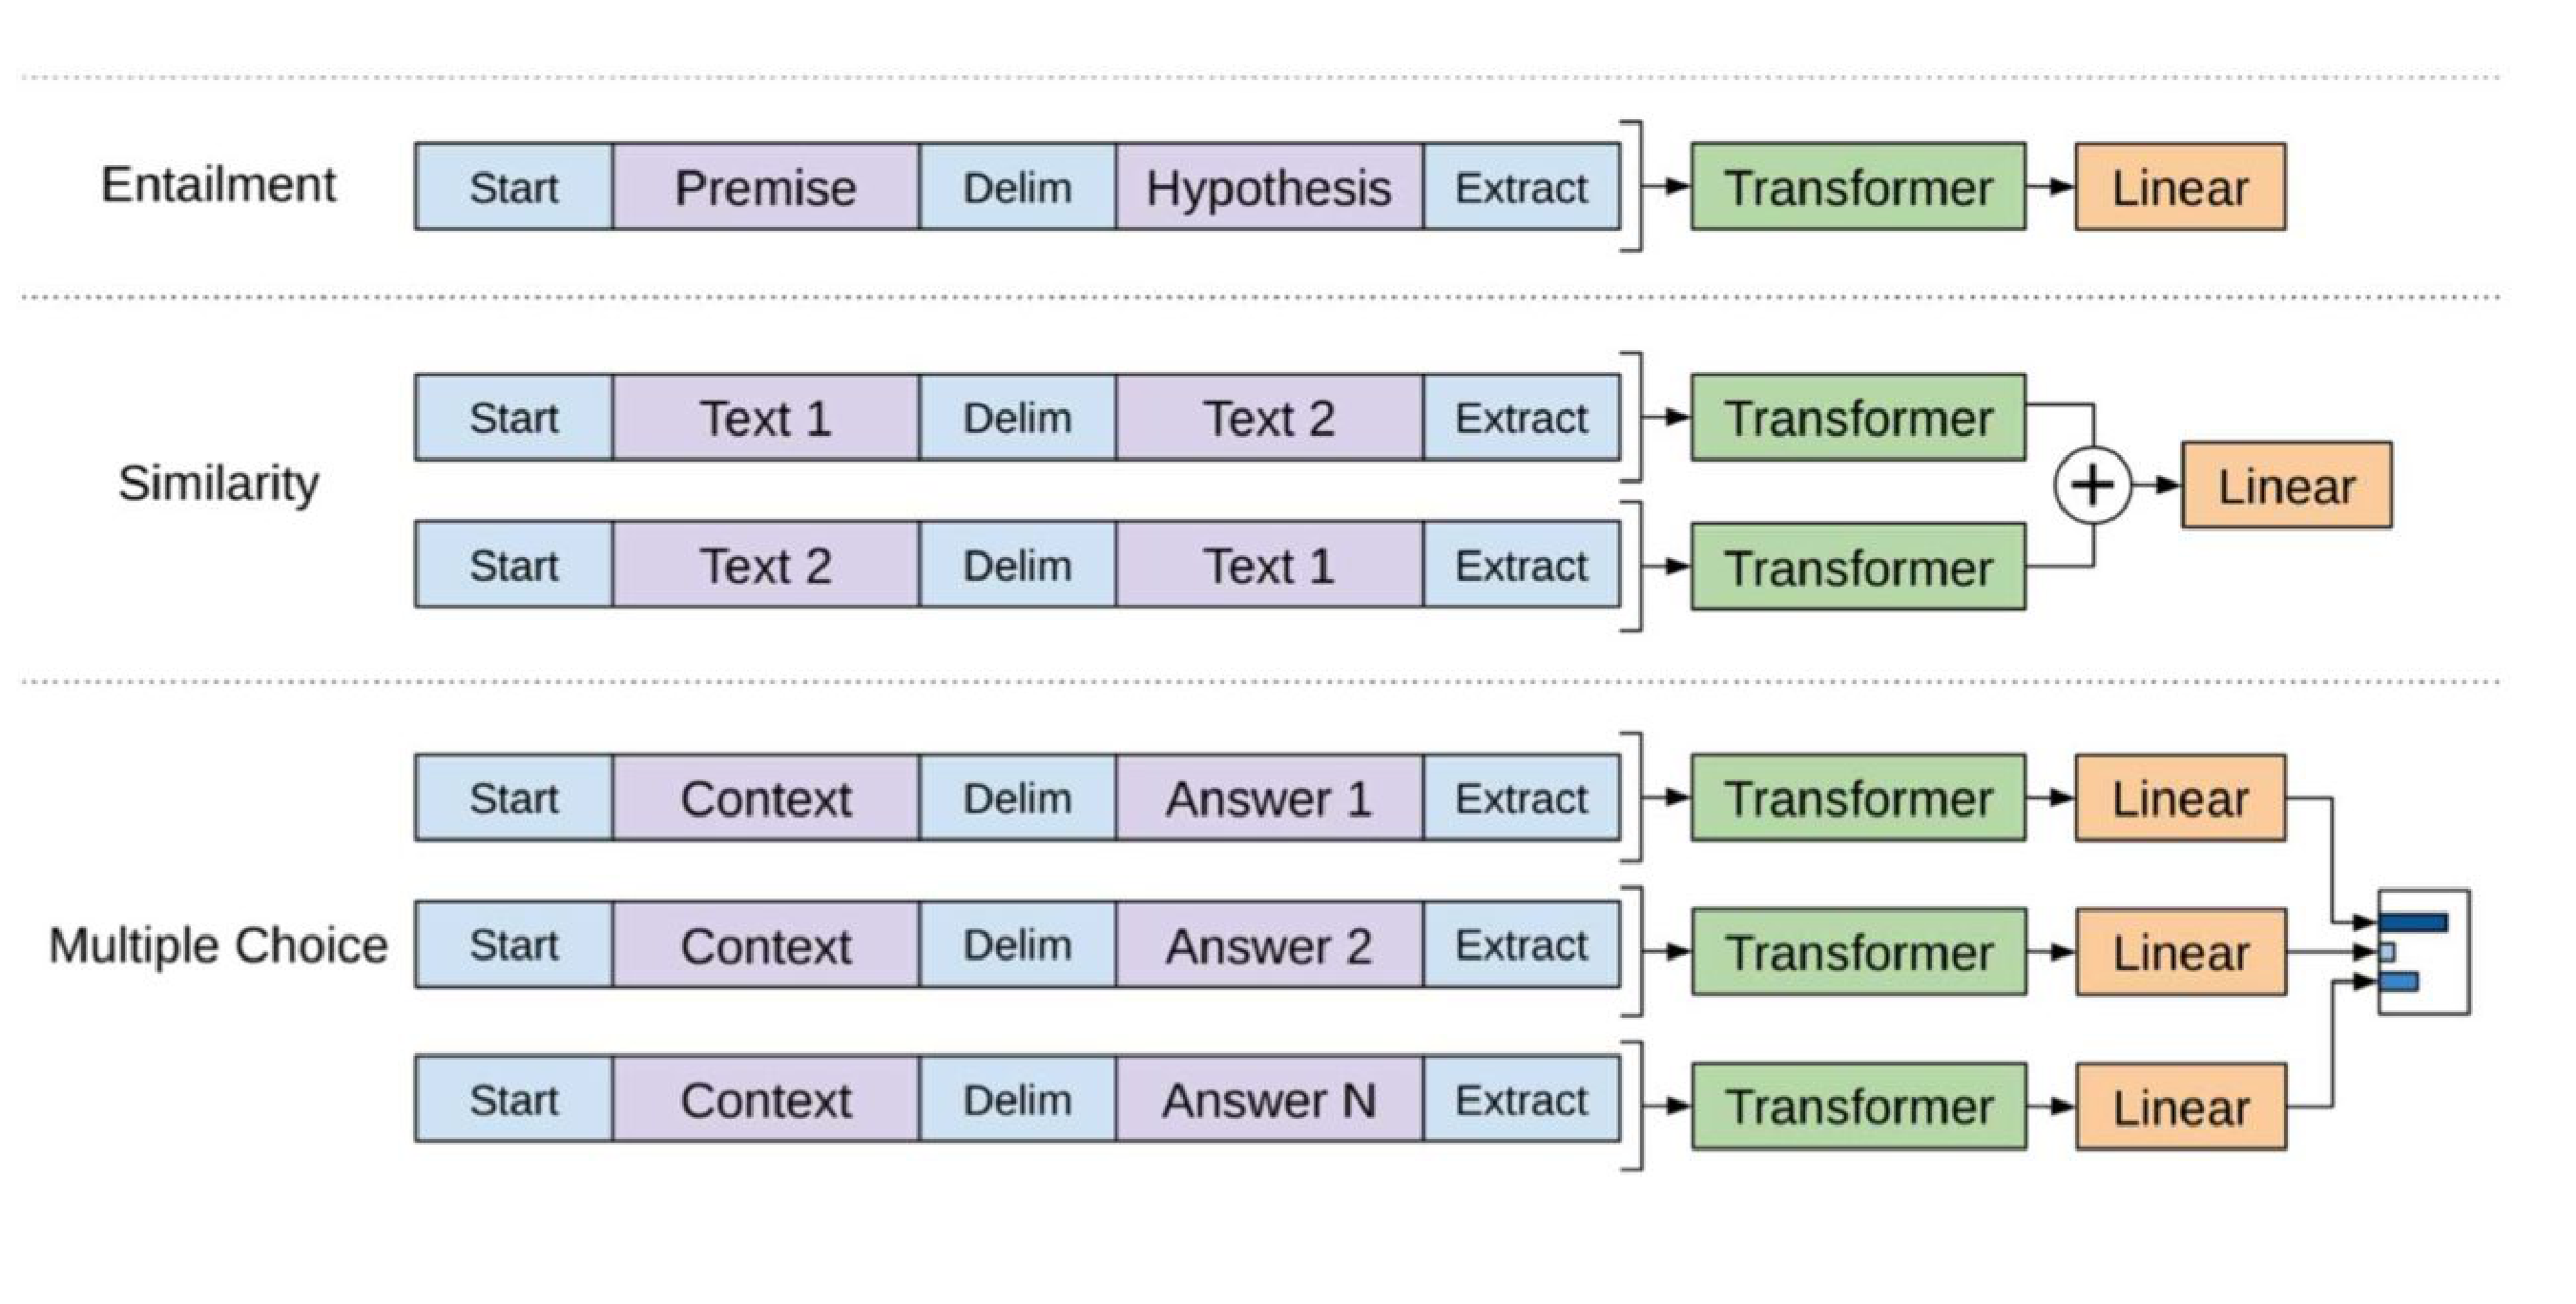
\includegraphics[width=0.9\textwidth]{figures/gpt.eps}

    \footnotesize{(Figure from \cite{radford2018improving}.)}
    
  \end{centering}  
\end{slide}

\begin{slide}[toc=BERT]{BERT (Google, 2018)}
  The next highly influential model was Google's BERT (Bidirectional Encoder
  Representations from Transformers, \cite{devlin2018bert}), whose main
  innovations were
  \begin{itemize}
  \item the use of two new self-supervised objectives instead of traditional
    language-modeling:
    \begin{itemize}
    \item masked language modeling, and
    \item next sentence prediction (NSP); and
    \end{itemize}
  \item a corresponding architectural change: the model is based on the
    \emph{transformer encoder} architecture.
  \end{itemize}
\end{slide}

\begin{slide}[toc=]{BERT: masked language modeling}
  The objective is to guess randomly masked tokens:\medskip
  
  \begin{centering}
    
    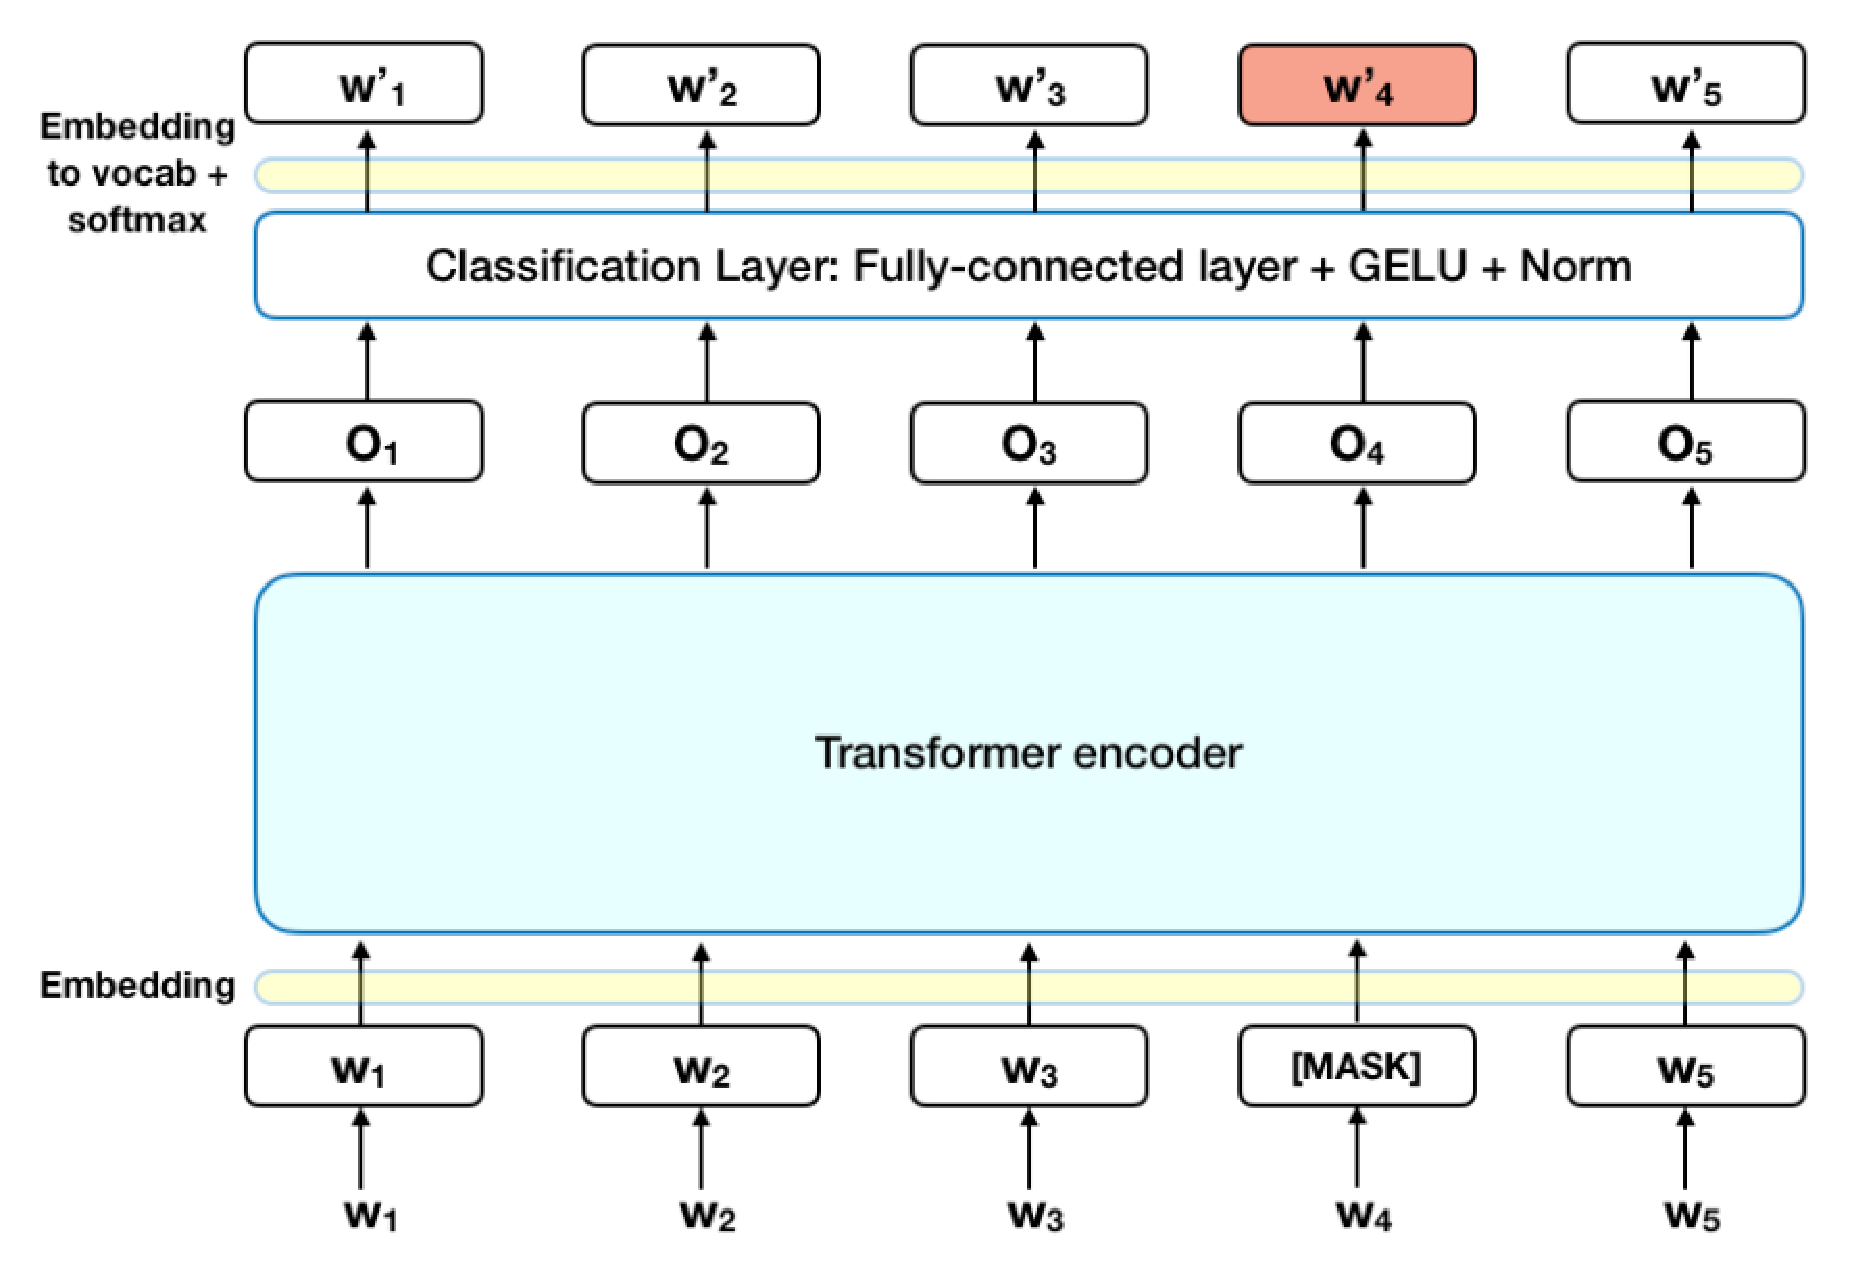
\includegraphics[width=0.9\textwidth]{figures/bert1.eps}

    \footnotesize{(Figure from \cite{horev2018bert}.)}
    
  \end{centering}
\end{slide}

\begin{slide}[toc=]{BERT: next sentence prediction}
  The second objective was deciding whether two sentences followed each other in
  the training corpus or were randomly sampled:\medskip
  
  \begin{centering}
    
    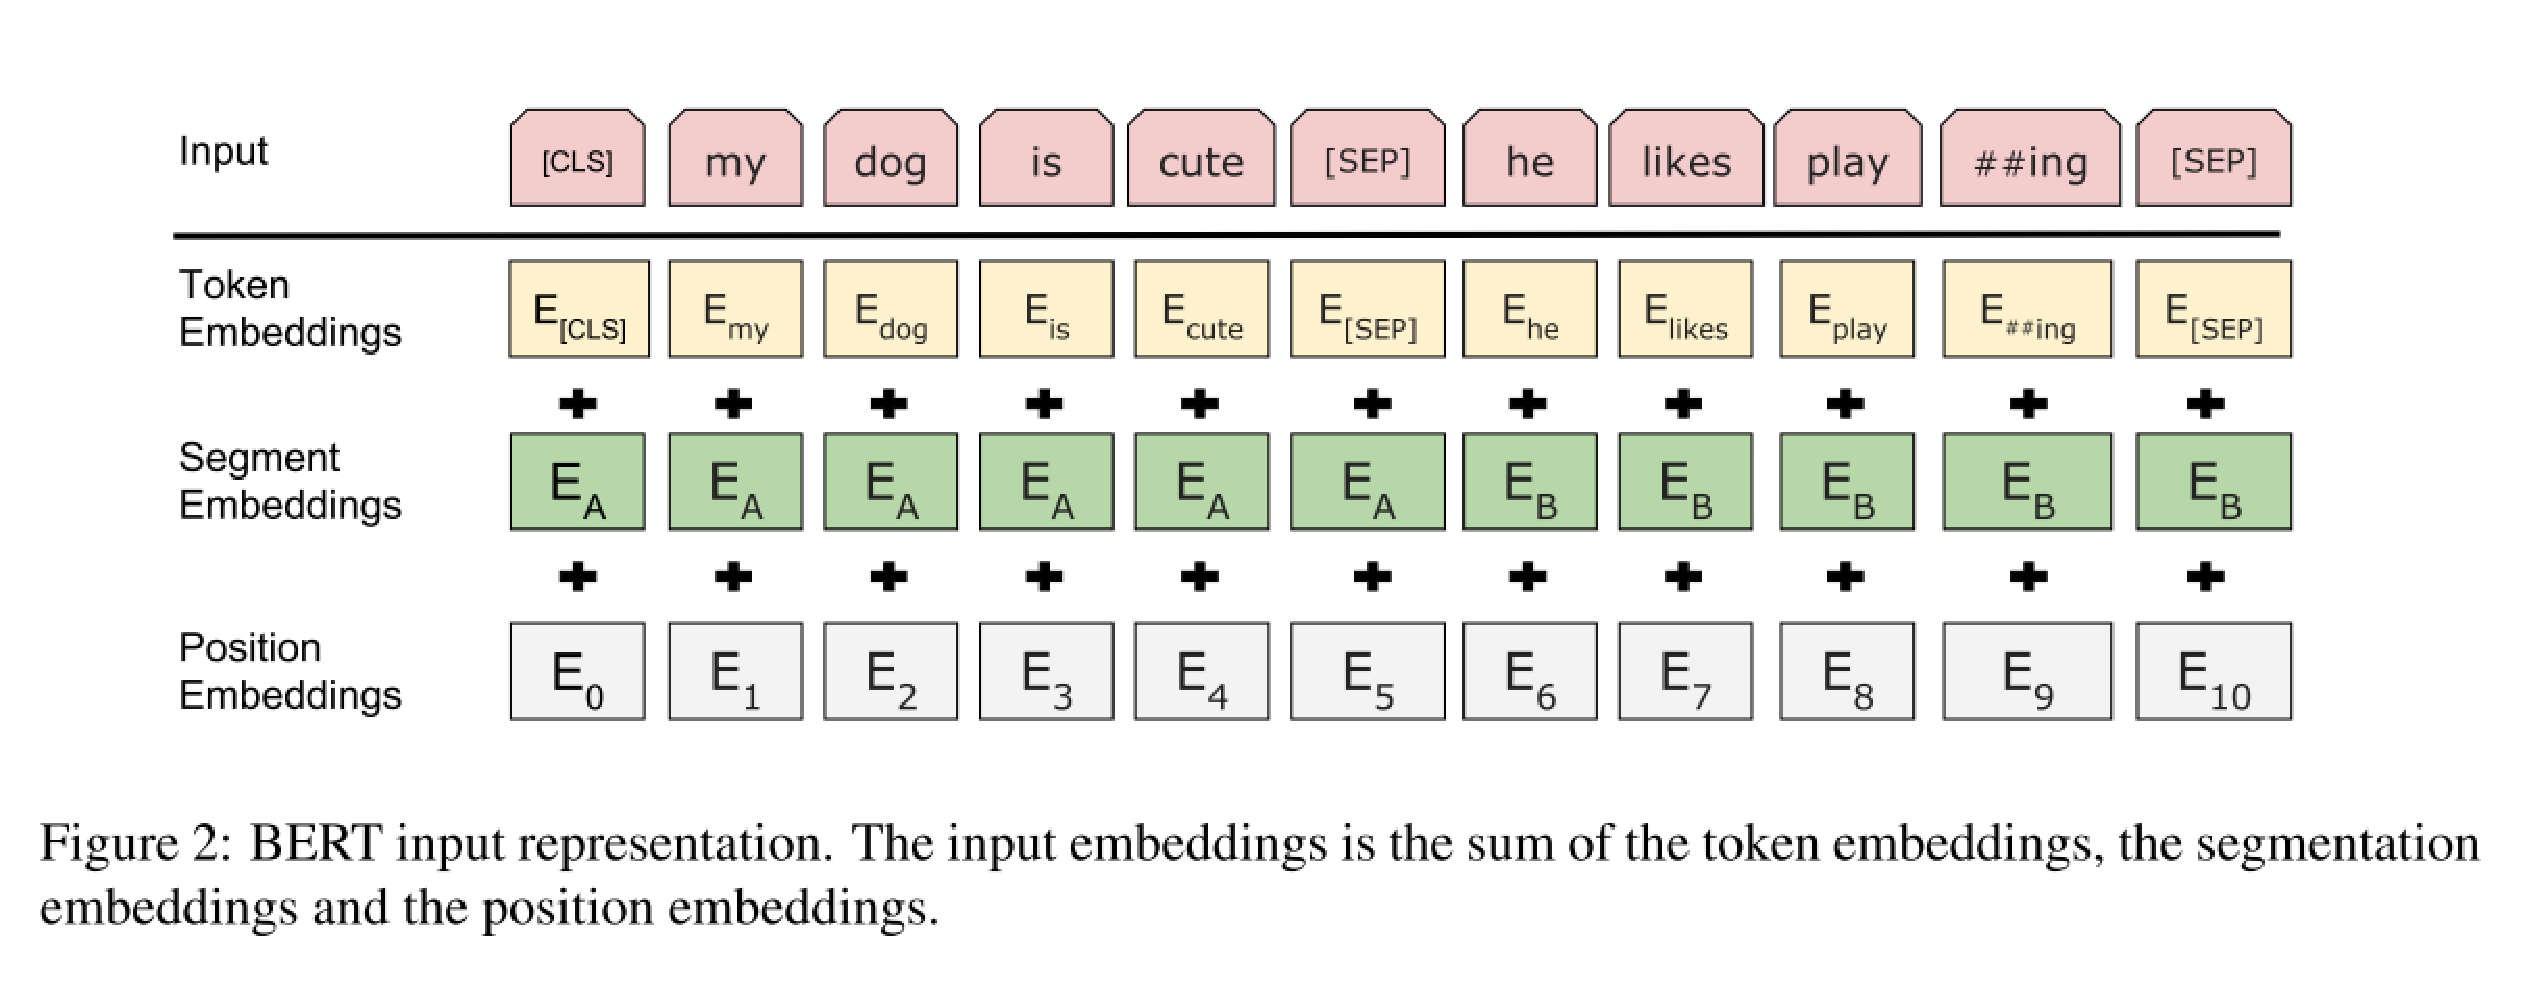
\includegraphics[width=1.\textwidth]{figures/bert2.eps}

    \footnotesize{(Figure from \cite{devlin2018bert}.)}
    
  \end{centering}
\end{slide}

\begin{slide}[toc=Recent trends]{Recent trends}
  Newer models have been able to improve on the state-of-the-art in NLP tasks
  again and again, but typically with an \emph{\gold increased number of
    parameters} and \emph{\gold on larger datasets}:\bigskip

  While the original ELMo model had 93.6 million parameters, GPT-3, the latest
  GPT version has 175 billion(!) parameters, and the dataset size increased from
  800 million to 300 billion tokens.
\end{slide}

\begin{slide}[toc=Distillation]{Knowledge distillation}
  The huge increases in size led to intensive research into \emph{knowledge
    distillation} methods to be able to produce smaller and more efficient
  models based on the original ones without significant performance
  loss.\bigskip

  A good example is \emph{\gold DistilBERT}, a distilled version of BERT trained
  to mimic BERT's output \citep{sanh2019distilbert}. DistilBERT retains 97\% of
  BERT's performance, but with 40\% fewer parameters and is 39\% faster during
  inference.
\end{slide}

\begin{slide}[toc=Sparse attention]{Sparse attention variants}
  Another way of improving efficiency has been reducing the scope of attention
  in the self-attention layers, since in full attention the number of dot
  products to be calculated is quadratic in the number of input tokens. Linear
  alternatives include
  \begin{itemize}
  \item \emph{\gold global attention}: a set of global tokens that attend to
    the whole sequence;
  \item \emph{\gold random attention}: for each query, a set of $r$ random keys
    is calculated to which that query attends;
  \item \emph{\gold window attention}: only local neighbors within a fix radius
    are attended to.
  \end{itemize}
\end{slide}

\begin{slide}[toc=Sparse attention]{Sparse attention variants cont.}
  The Big Bird contextual embedding model \citep{zaheer2020big} combines all
  these linear attention types to increase the number of input tokens
  significantly without significant change in memory requirements:\medskip

  \begin{centering}
    
    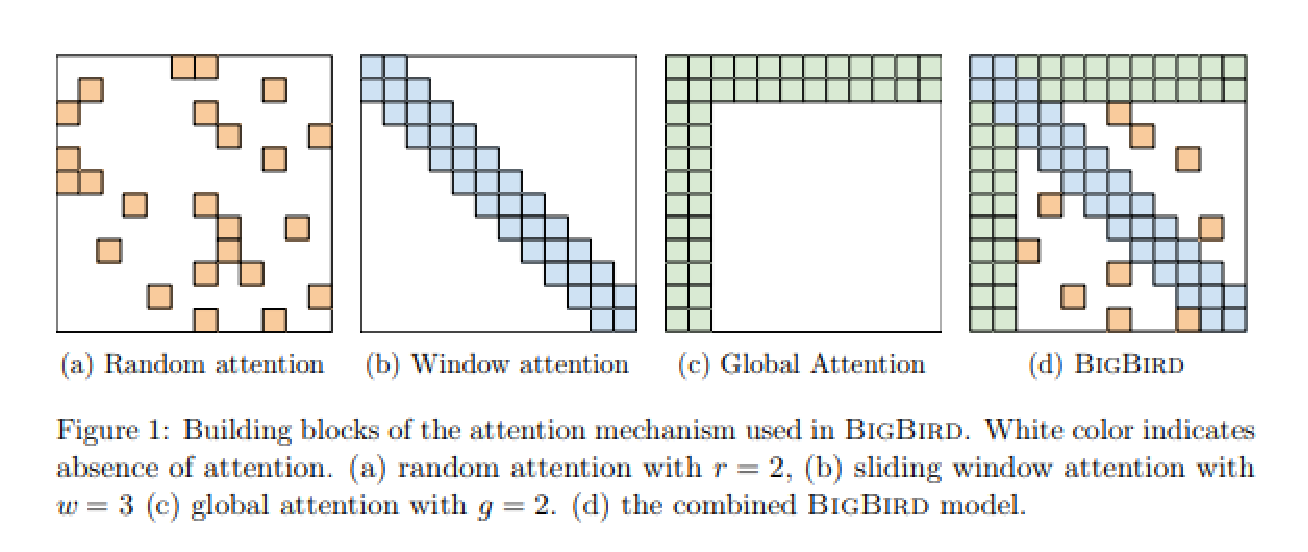
\includegraphics[width=1.\textwidth]{figures/bigbird.eps}

    \footnotesize{(Figure from \cite{zaheer2020big}.)}
    
  \end{centering}
\end{slide}

\begin{slide}[toc=Few-shot learning]{Few- one- and zero-shot learning}
  An interesting research direction is to try to use the model directly, without
  added layers and gradient updates on downstream tasks. Some recent models,
  most importantly, GPT-3 \citep{brown2020language} can perform surprisingly
  well on various downstream tasks that are explained in the input. There are
  three learning settings:
  \begin{itemize}
  \item \emph{\gold zero-shot}: The input only contains a short description of
    the supervised task, and a concrete input instance prompt , e.g. ``Translate
    English to French: cheese =$>$ ''.
  \item \emph{\gold one-} and \emph{\gold few-shot}: In addition to the short
    task description, the input also contains one or a few training examples
    before the prompt.
  \end{itemize}
  
\end{slide}

\section {References}

\begin{slide}{References}
  \bibliographystyle{plainnat}
  \nobibliography{nlp_course.bib}
  \begin{footnotesize}

    \bibentry{akbik2018contextual}.\medskip

  \end{footnotesize}
\end{slide}

% \begin{slide}[toc=]{References cont.}
%   \begin{footnotesize}

%     \bibentry{peters2018deep}.\medskip
    
%   \end{footnotesize}
% \end{slide}

\end{document}

%%% Local Variables:
%%% mode: latex 
%%% TeX-master: t
%%% End:

% LocalWords:  Tokenization Discriminative discriminative
